\documentclass[a4paper, 11pt, onepage]{scrreprt}

\usepackage{fontspec}
\setmainfont{Linux Libertine O}
\usepackage{polyglossia}
\usepackage{amssymb}
\usepackage{amsmath}
\usepackage{xfrac}
\usepackage{mathtools}
\usepackage{bbold}
\usepackage[hyperref]{xcolor}
\usepackage{graphicx}
\usepackage{listings}
\usepackage{caption}
\usepackage{wrapfig}
\usepackage{float}
\usepackage{tabularx}
\usepackage{booktabs}
\usepackage{numprint}
\usepackage{hyperref}
\usepackage{siunitx}

\newcommand\wiki{\textsc{Wikipedia}}
\newcommand\ew{\textsc{English Wikipedia}}
\newcommand\sew{\textsc{Simple English Wikipedia}}
\newcommand\tableref[1]{\hyperref[#1]{Table \ref*{#1}}}
\newcommand\figureref[1]{\hyperref[#1]{Figure \ref*{#1}}}
\newcommand\sectionref[1]{\hyperref[#1]{Section \ref*{#1}}}
\newcommand\chapterref[1]{\hyperref[#1]{Chapter \ref*{#1}}}
\newcommand\equaref[1]{\hyperref[#1]{Equation \ref*{#1}}}
\newcommand\maps[1]{\xrightarrow{\mathcal{#1}}}
\newcommand\card[1]{\lvert #1 \rvert}
\newcommand\suchthat{\, \middle| \,}
\newcommand\given{\, \middle| \,}
\newcommand\proba[2][]{P_{#1} \left( #2 \right)}

\DeclareMathOperator*{\argmin}{\arg\,\min}
\DeclareMathOperator*{\argmax}{\arg\,\max}

\renewcommand\chaptername{Section}
\renewcommand\thechapter{\Roman{chapter}}

\DeclareGraphicsExtensions{.png, .jpeg, .jpg, .svg, .eps, .pdf}
\graphicspath{{./img/}}

\hypersetup{
  colorlinks = true,
  linkcolor = violet,
  urlcolor = teal,
  citecolor = gray
}

\begin{document}
\begin{titlepage}
  \begin{center}
    \noindent\rule{\textwidth}{0.4pt}
    {\huge\bfseries Improving text readability using\\
      \sew\\}
    \noindent\rule{\textwidth}{0.4pt}\\
    % ----------------------------------------------------------------
    \vspace{1.5cm}
    {\large
    \begin{tabularx}{\textwidth}{lXll}
      \textbf{Author:} & \textsc{Hugo Mougard} &
      \textbf{Director:} & \textsc{Akiko Aizawa} \\
      \textbf{Tutor:} & \textsc{Colin de la Higuera} &
      \textbf{Advisor:} & \textsc{Pascual Martínez-Gomez} \\
    \end{tabularx}}\\[5pt]
    % ----------------------------------------------------------------
    \vfill
    \parbox{0pt}{\large \begin{tabbing}
        \textbf{Sending institution:} \= National Institute of Informatics \kill
        \textbf{Sending institution:} \> \textsc{Université de Nantes, France} \\
        \textbf{Hosting institution:} \> \textsc{National Institute of
        Informatics, Japan} \\
      \end{tabbing}}
    \vfill
    {\LARGE ATAL Master 2 internship report}
    \vfill
    % ----------------------------------------------------------------
    
\includegraphics[width=0.16\textwidth]{img/nii.png}
    \hspace{0.03\textwidth}\hfill
    
\includegraphics[width=0.19\textwidth]{img/lina.png}
    \hfill
    
\includegraphics[width=0.19\textwidth]{img/univ.eps}
    \vfill
    {July 2014}
  \end{center}
\end{titlepage}

\tableofcontents

\chapter{Acknowledgments}

I would like to start those acknowledgments by thanking Aizawa-sensei
and Katsu-san for their precious help before our arrival to Japan, and
their tireless support during our stay, this was greatly appreciated.

Meeting a solid number of great people has been a pleasure during this
internship. I thank especially Fujinuma-san and Adelin for their
support (and corrections to this report for the latter).

I also wouldn't have been able to conduct this internship without the
scientific advising of Aizawa-sensei and Pascual-san, I thank them for
all their good insight, even though I am convinced I didn't make the
best of it.

And it was very nice to have someone exterior to discuss ideas with
when I wanted to, I thank Colin de la Higuera for that.

Because this internship is also the end of my Master's program, I
would like to acknowledge the awesomeness of the ATAL team (students
and teachers alike!). Working with passionate people in this context
has been a pleasure for now close to two years.

Lastly but not leastly—please forgive my English, I would like to
thank Grégoire for about everything during those five months of
internship, it was great to share this Japanese experience with a
friend (and still will be for about three weeks at the
time of this writing).

\chapter{Laboratory presentation}

\section{\textsc{National Institute of Informatics}}
\label{sec:national-institute-of-informatics}

The \textsc{National Institute of Informatics} is a Japanese research
institute located in Chiyoda-ku, Tokyo. It has strong connections with
the \textsc{University of Tokyo} (\textsc{Todai}) and welcomes
computer scientists of numerous domains to form a strong innovative
pole in the Japanese computer science research landscape.

Its International Exchange Agreements program allowed myself and
another student of the first promotion of the ATAL master to join for
a five month internship.

\section{\textsc{Aizawa Laboratory}}
\label{sec:aizawa-laboratory}

The team that welcomed me for this work is \textsc{Aizawa
  Laboratory}\footnote{\url{http://www-al.nii.ac.jp/en/}}. It is led
by Professor \textsc{Akiko
  Aizawa}\footnote{\url{http://research.nii.ac.jp/~akiko/index_e.html}},
the director of this internship. At the time of this writing, the
laboratory has 18 members and strong partnerships with past members of
the laboratory.

Its expertise lies in several sub-domains of Natural Language
Processing (NLP):
\begin{itemize}
\item NLP using gaze information;
\item analysis and mining of scientific papers;
\item mathematical information retrieval;
\item syntactic and semantic structure analysis of natural language
  text;
\item extraction and classification of technical terms.
\end{itemize}

The work presented in this report has been done in the group
interested in NLP using gaze information, mostly for historical
reasons: the work proposed during this internship doesn't use gaze
information. Still, readability — the topic of this internship — has
strong connections to gaze NLP and other members of the group were
very knowledgeable in this domain. This was a great opportunity for
the development of this internship.

\chapter{Introduction}

Whether it is to teach children how to read, to assess the
comprehensiveness of technical manuals or to better grasp how we
understand things, readability has been studied for about two
centuries for its impact in both engineering and scientific endeavors.

Despite the interest of the scientific community for many aspects of
readability—including cognitive and social ones, early research was
mostly focused on finding basic metrics to measure how understandable
a text is. It is only in recent years that scientists have been able
to come up with more interesting methods, thanks in particular to the
advances in machine learning, gaze processing, the new speed of modern
computers and the unparalleled amount of data available on the
internet.

The high-level goal of this internship is to investigate these methods
and improve on them. To be more specific, most methods consider
documents as a whole when analyzing their readability, which makes it
hard for users to understand which parts are the most important to
rework. We aim at providing a fine-grained analysis of readability in
this work. This shift towards fine-grained analysis of linguistic
phenomena has been observed in recent years in other natural language
processing domains, such as sentiment analysis with the recursive
approach proposed by \cite{socher2013recursive} that allows users to
detect which part of a sentence conveys which sentiment. In the same
way, we want to detect which part of a sentence is readable or non
readable, and for which reasons.

\chapter{Related work}
\label{cha:sota}

This section details the history and state of the art of computational
readability study that served as a basis for this work.

\section{Early works and readability formulas}
\label{sec:early-works-and-formulas}
Readability has been studied extensively. The first works in this area
date back to more than a century ago: in 1893, Sherman published a
book \cite{sherman1893analytics} where he compared modern English and
English spoken four centuries before with considerations that are very
alike the ones that current readability studies outline. Then, in
1921, Thorndike computed a list of ten thousand easy-to-read words
\cite{thorndike1921teacher}. This list got used shortly thereafter by
teachers trying to select good books for children learning to read
\cite{lively1923method}: they went through the process of estimating
the readability of many books thanks to a basic formula and
Thorndike's list.

This was the beginning of an important branch of research focusing on
how to best estimate the readability of a text thanks to simple
formulas. Among the most famous methods, it is interesting to mention
the Flesch Reading Ease \cite{flesch1948new} which introduced the use
of a combination of the average number of words per sentence and the
average number of syllables per word to estimate the readability of a
text. Most of the subsequent approaches also use those metrics. This
method yields a 0.91 correlation with text understanding and has been
used outside of research to improve the readability of a vast amount
of publications, yielding excellent results in readership increase.

Roughly at the same time, Dale and Chall introduced a readability
formula that makes use of a list a words instead of the average number
of syllables per word to estimate readability
\cite{dale1948formula}. This more precise definition of world
difficulty allows this metric to reach a 0.93 correlation with text
understanding and because of that has been one of the most used
formulas in research.

Later works brought formulas that are easier to compute or give
slightly better results. These improvements were not small
improvements due to the time required to compute readability formulas
on a large number of texts at the time. Some also give their result as
the grade that would be required to be able to read the input
text. Overall, all are using the same variables as either Flesch or
Dale and Chall \cite{mclaughlin1969smog, kincaid1975derivation,
  chall1995readability}.

Despite their useful applications, readability formulas are not
perfect. Some works have detailed their problems convincingly
\cite{duffy1985readability, schriver2000readability}. Among the most
important ones is the imprecision of the features used: of the
following sentences, (1.)  is often considered easier to understand
than (2.), despite being lengthier:
\begin{enumerate}
\item The mouse ate the cheese, and then the rat ate the mouse, and
  after that, the cat ate the rat and died.
\item The cat that ate the rat that ate the mouse that ate the cheese
  died.
\end{enumerate}
That showcases that sentence length should be considered with care
when trying to improve on existing readability measures. The average
word length—one of the other dominant features—has similar
problems. The reasons for that is two-fold:
\begin{itemize}
\item affixes are known even to early readers;
\item some very short words are difficult intrinsically.
\end{itemize}
To illustrate that we can compare “curr” (to make a murmuring sound)
and “reinventing”. Due to the rarity of “curr”, most early readers
will have troubles with it while “reinventing” will often not be
problem because of the known meanings of the “re-” and “-ing” affixes.

Finally, the fact that many formulas only consider short windows of a
text to estimate its readability make them not reliable without
repetition of the measure at several points in a text and an averaging
(which is what Dale \& Chall does by default).

To address those shortcomings, scientists have recently proposed
machine learning based approaches. The next section details those
works.

\section{Machine Learning approaches}
\label{sec:ml-approaches}

Readability assessment can be seen as a supervised classification
task. To predict the required grade to understand a given input text,
\cite{collins2004language} use a unigram language model of each target
grade in order to see which one is the most likely to generate the
input.

\cite{schwarm2005reading} improve on this approach by using a trigram
model instead of a unigram model. They also incorporate classical
readability features by using a SVM with the perplexity scores of the
language models as features along with readability formula scores and
various syntactic features.

In 2008, Pitler and Nenkova conduct a study where they further
investigate the use of complex features to feed machine learning
readability approaches \cite{pitler2008revisiting}. They study
features such as discourse relations and entity coherence together
with advanced syntactic and lexical features. They notice possible
improvements but conclude that until robust automatic method to obtain
the more advanced features exist, it is unlikely that people will
succeed in using them in a large scale, automated system.

With machine learning approaches becoming successful, gathering data
became a crucial point of readability research. In the next section we
see how researchers have used \wiki{} to conduct their machine
learning research in readability.

\section{Readability research using \wiki}
\label{sec:wiki-approaches}

From 2006 onwards—since its inception—\sew{} has been rightly seen as
an important resource for readability studies. Scientists have used it
to compute parallel corpora of readable sentences and their
hard-to-read counterparts.

Among the most notable works, \cite{zhu2010monolingual} used the
comparable nature of \wiki{} and \sew{} to compute a parallel corpora
about readability and proposed a general rewriting model based on tree
transduction to exploit their corpus.

Following the approach proposed by \cite{nelken2008mining} in the
compression domain, in \cite{yatskar2010sake, woodsend2011learning},
\sew{} is used as a basis to compute a parallel corpus on its own,
thanks to its revision history. The corpora obtained are then used to
train lexical simplification systems in the case of
\cite{yatskar2010sake} and general systems
\cite{woodsend2011learning}.

\cite{biran2011putting} take a different look at the problem. They
learn simplifications thanks to \wiki{} and \sew{} but without
computing a parallel corpus. Instead, they rely on a set of methods to
simplify words while preserving grammaticality. They also take word
contexts into account thanks to a classical context vector method.

Another interesting work using \sew{} is \cite{wubben2012sentence}. It
considers text simplification as a monolingual machine translation
task. This approach has important similarities with the use of machine
translation in the paraphrasing task.

\chapter{Work}
\label{cha:work}

To achieve fine-grained readability analysis, we propose an approach
relying on statistical phrase based translation
\cite{koehn2003statistical}. The underlying idea is to build a lexicon
of not-so-readable phrases and their readable counterparts along with
scores reflecting the quality of the pairings. This lexicon can then
be used to score areas of a text depending on the translations
available for them, yielding a fine-grained readability assessment of
a text. \sew{} is used as a corpus to build such a lexicon. The
process used is detailed in the first section of this chapter.

In the literature, most of the best translation models are based on a
language model of the target language. In this approach, we extend
this model to also consider the source language to better fit the
readability simplification problem. This extension is the object of
the second section of this chapter.

As mentioned above, with such a model defined, it is possible to
create a fine-grained measure to assess the readability of a text. The
details of this operation are exposed in the third section.

The following section will then look at how to rewrite texts from the
models computed beforehand and finally, the last section of this
chapter introduces a tool—\textsc{Readability Lab}—created to explore
the results of our approach.

\section{Automatic readability parallel corpus creation}
\label{sec:corpus}

Machine learning approaches are used more and more and in a wide range
of scientific domains for their effectiveness. Most of the time, the
more data you have, the best your results will be, up to an extent
that people described data efficiency as “unreasonable”
\cite{halevy2009unreasonable}. In this context, it seems that being
able to automatically gather data is of utmost importance. Moreover,
raw data is often not enough. Most techniques require a lengthy and
costly annotation process. For this reason, researchers in every
domain using machine learning invest time finding clever techniques to
automatically obtain annotated corpora.

In readability, such a clever technique is to leverage the power of
\wiki, and in particular \sew. To do so, mainly two techniques have
been used: the first is to align the articles present both in the
regular \ew{} and in \sew{} to build a parallel corpus. This approach
has been used with great success in \cite{zhu2010monolingual} and has
resulted in the
\textsc{PWKP-108016}\footnote{\url{https://www.ukp.tu-darmstadt.de/data/sentence-simplification/simple-complex-sentence-pairs/}}
dataset. The second is to use the revision history of \sew, as
showcased in \cite{yatskar2010sake}. In this work we use the second
approach.

The main rationale for not using the existing \textsc{PWKP-108016}
corpus and instead creating one of our own is that we believe the
technique used to automatically construct the corpus from a revision
history is a general process and can therefore be extended to many
data sources beyond \wiki. Hence the community would benefit from an
efficient tool to exploit such sources. Those possible extensions
include many of the processes of the professional publishing world and
especially copy editing. If proven efficient, big corpora could be
gathered from journalists, writers, scientists, etc. On the contrary,
it has been shown to be extremely hard to find good comparable corpora
outside of \wiki{} and some restricted institution publications such
as the European Parliament proceedings on which \textsc{Europarl} is
based \cite{koehn2005europarl}, which makes the first approach hard to
generalize. It is worth noting that it might be even harder to
construct such corpora for readability study than for machine
translation, due to the lesser number of publications requiring
different levels of readability than the number of publications that
need to be translated. Finally, the outputs made public by
\cite{yatskar2010sake} are of high quality but not intended to be used
as a corpus and rather as a supplementary material to study their
approach.

To build automatically our corpus, we leverage the fact that when
editing \sew, contributors have the possibility to write a commit
message, so that other people can quickly browse history and guess the
role of a particular commit. This allows us to automatically detect if
a particular commit was intended to fix a readability issue or was
serving another purpose (improving the content of the article,
cleaning the wiki, vandalizing, …). This usage of metadata is not
novel, it was used in the \textsc{Simpl} approach presented in
\cite{yatskar2010sake}. Though, we fine-tune the heuristic used to
address some problems encountered in this article and to harden the
process. An example of readability edit can be seen in
\figureref{fig:dan-kelly}.

\begin{figure}[H]
  \centering
  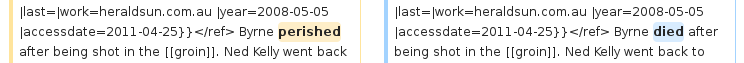
\includegraphics[width=\textwidth]{dan-kelly}
  \caption{An edit of the Dan Kelly article with the commit message
    “use simple english here”}
  \label{fig:dan-kelly}
\end{figure}

The heuristic we use to gather edits is extremely simple: as a first
step, the category information of a commit is removed. For example, in
the commit message “/* Casablanca */ make the movie description more
readable” the part “/* Casablanca */ ” is automatic data added by the
\textsc{Mediawiki} software to specify in which section the edit was
made. Once this part of the commit is deleted, we only consider commit
messages $m$ so that:

\[
m \in \left\{\text{“simplify”}, \text{“simplifying”},
  \text{“simplified”}, \text{“simplification”},
  \text{“simpler”}\right\}
\]

This may seem drastic but we believe it is necessary due to the many
noisy commits introduced with broader rules. To illustrate this point,
we can consider the commit messages of
\tableref{tab:problematic-commits}. We can see that commit \#1 has two
purposes, one of which will bring noise (the wikification). Commit \#2
contains one of the matching terms, but we should not consider
it. It's not clear if commit \#3 tries to address readability or not.

\begin{table}[h]
  \centering
  \caption{Problematic commit messages}
  \begin{tabular}{rp{12cm}}
    \toprule
    \# & Commit message \\
    \midrule
    1 & “simplified, and wikified” \\
    \addlinespace
    2 & “wikify. needs simplifying” \\
    \addlinespace
    3 & “exhaustive, to help us work out titles of articles - lots of
    discussion here, and no, this is not simple engouh yet” \\
  \end{tabular}
  \label{tab:problematic-commits}
\end{table}

Furthermore, we determined by an empirical study that those commits
represented an important part of the commits we might have retrieved
with a broader rule, so we simply did not consider them.

The next step for the creation of the corpus is to compute the precise
edit that the contributor made. To do so, tokenization and sentence
splitting both were performed on the original version of the article
and its revision using
\textsc{OpenNLP}\footnote{\url{https://opennlp.apache.org/}}. Then the
two texts were aligned at the word and sentence levels with Myers'
alignment algorithm—the algorithm used in git to compute diffs
\cite{myers1988optimal}. We rely on the implementation proposed by
\textsc{jgit}\footnote{\url{http://www.eclipse.org/jgit/}}.

Keeping re-usability in mind, the implementation uses
\textsc{uimaFIT}, a standard NLP framework
\cite{ogren-bethard:2009:SETQA-NLP}. The complete pipeline is
available on
\textsc{Github}\footnote{\url{https://github.com/m09/readability}}. It
is freely re-usable thanks to its permissive license.

The obtained corpus—which has \numprint{43753} entries—has important
noise problems. A quick glance at \tableref{tab:problematic-edits} is
sufficient to understand that some edits are not readability edits,
but either alignment deficiencies or edits serving complementary
roles. When filtered to only consider revisions of 5 words at most, to
match the policy used in \cite{yatskar2010sake}, the number of entries
is reduced to \numprint{35927}. Of those \numprint{35927} couples
$(\mathtt{original}, \mathtt{revision})$, \numprint{25675} occur only
once and \numprint{18330} $\mathtt{original}$s have only one readable
equivalent.

\begin{table}[H]
  \centering
  \caption{Problematic edits}
  \begin{tabular}{rp{6cm}p{6cm}}
    \toprule
    \# & Original version & Revised version \\
    \midrule
    1 & , and & . she also used them in her arguments about \\
    \addlinespace
    2 & 2010 federal election, is russell matheson, a member & size\\
  \end{tabular}
  \label{tab:problematic-edits}
\end{table}

The resulting resource is enriched with part-of-speech, and syntactic
parsing annotations and is proposed in an XML format.

\section{Phrasal lexicon creation}
\label{sec:lexical-enhancements}

The corpus $\mathcal{C}$ created in \sectionref{sec:corpus} can be
used as a basis for phrase based translation, in order to simplify
vocabulary in a text. The goal is to allow authors to pick simpler
words than the ones they used, in an efficient manner. With
$\mathcal{P}$ denoting the multiset of all english phrases, we
consider $\mathcal{C} \subset \mathcal{P} \times \mathcal{P}$ as a
multiset of lexical pairs $(x, y)$ where we found in \sew{} that $x$
was rewritten into $y$.

To reduce lexical ambiguity, phrases are matched with their part of
speeches. This way, “it was a good \emph{buy}.” and “I \emph{buy} it.”
will not have their translations mixed.

A score function $\mathcal{S} : \mathcal{P} \times \mathcal{P}
\rightarrow \mathbb{R}$ is needed to turn the corpus $\mathcal{C}$
into a phrasal lexicon $\mathcal{L} \subset \mathcal{P} \times
\mathcal{P} \times \mathbb{R}$. To design such a function, there are
two properties to satisfy that are of utmost importance:

\begin{itemize}
\item giving more importance to $(x, y)$ if $x$ is not a common word:
  the less common a word is, the more important it is to rewrite it;
\item giving more importance to $(x, y)$ if $y$ is a common word to
  end up with the simplest translations ranked at the top.
\end{itemize}

We use a language model on one hand and probabilities to assess the
commonness of a rewriting in $\mathcal{C}$ on the other hand to
properly model those properties. The language model is built on the
final version of every harvested page of \sew, at a bigram level.

$\mathcal{S'}$ is now introduced as the first combination proposed of
these two elements. It will serve as a basis for some variations
presented later on in this section. The probability of a rewriting
occurring in $\mathcal{C}$ is defined in \equaref{eq:prob} in terms of
the size of the two multisets concerned:

\begin{align}
  \label{eq:prob}
  \proba[\mathcal{C}]{(x, y)} & = \frac{\card{\left\{(x, y) \suchthat
        (x, y) \in \mathcal{C}\right\}}}{\card{\mathcal{C}}} \\
  \label{eq:s'1}
  \mathcal{S'}((x, y)) & = \log \frac{\proba[\mathcal{C}]{(x, y)}^{\lambda_1}}%
  {\proba[LM]{x}^{\lambda_2}} \\
  \label{eq:s'2}
  & = \lambda_1 \log \proba[\mathcal{C}]{(x, y)} - \lambda_2 \log \proba[LM]{x}
\end{align}

This function works on logs to ensure the numerical precision of the
computations despite the imprecision of floating point arithmetic for
small values.

The view of the problem we express with the design of $\mathcal{S'}$
is that a strong rewriting is a frequent rewriting of a rarely
occurring word. The two equations above explain this in two different
ways. \equaref{eq:s'1} best shows that $\mathcal{S'}$ is an
approximation of the ratio of the number of times a word is rewritten
on the number of times it appears in English. \equaref{eq:s'2} best
shows that $\mathcal{S'}$ is a balancing act: both $\log
\proba[\mathcal{C}]{(x, y)}$ and $\log \proba[lm]{x}$ are negative
quantities: by subtracting one to the other we balance two properties
of a good rewriting. $\lambda_1$ and $\lambda_2$ are parameters to
control this balancing.

Instead of defining the frequency of a rewriting from $x$ into $y$ as
the global frequency of $(x, y)$ in the corpus $\mathcal{C}$, it is
interesting to define it as the conditional frequency given that $x$
is being rewritten. This definition is well captured by the
conditional probability defined in \equaref{eq:probcond} and its
application to the score $\mathcal{S'}_{c}$ defined in
\equaref{eq:s'c}. $c$ stands for “conditional”:

\begin{align}
  \label{eq:probcond}
  \proba[\mathcal{C}]{(x, y) \given x} & = \frac%
  {\card{\left\{(x, y) \suchthat (x, y) \in \mathcal{C}\right\}}}%
  {\card{\left\{(x, y') \suchthat y' \in \mathcal{P} \land (x, y') \in
        \mathcal{C}\right\}}} \\
  \label{eq:s'c}
  \mathcal{S'}_{c}((x, y)) & = \log \frac%
  {\proba[\mathcal{C}]{(x, y) \given x}^{\lambda_1}}%
  {\proba[LM]{x}^{\lambda_2}}
\end{align}

The scores $\mathcal{S'}$ and $\mathcal{S'}_c$ already have
nice qualities to model different definitions of good rewritings. But
as they stand, the lengthier the word being rewritten, the better the
score of its rewriting, almost regardless of whether or not the
rewriting is a good lexical rewriting. This happens because the
language model probability of a $(n+1)$-gram is almost always an order
of magnitude lower than the language model probability of a
$n$-gram.

Concretely it means that the rewriting of a bigram such as “\emph{,
  and} $\rightarrow$ \emph{.}”  will come above most lexical
rewritings, such as the rewriting “\emph{exhausted} $\rightarrow$
\emph{tired}”. Taking into account the length of the sequence being
rewritten allows to fix that. The scoring functions $\mathcal{S}$ and
$\mathcal{S}_c$ are extensions of respectively the scoring functions
$\mathcal{S'}$ and $\mathcal{S'}_c$ and are introduced to average the
language model scores by considering the length of the words
considered. $w$ stands for “weighted”:

\begin{align}
  \label{eq:s}
  \mathcal{S}((x, y)) & = \log \frac%
  {\proba[\mathcal{C}]{(x, y)}^{\lambda_1}}%
  {\sqrt[\card{w}]{\proba[LM]{x}}^{\lambda_2}} \\
  \label{eq:sc}
  \mathcal{S}_{c}((x, y)) & = \log \frac%
  {\proba[\mathcal{C}]{(x, y) \given x}^{\lambda_1}}%
  {\sqrt[\card{x}]{\proba[LM]{x}}^{\lambda_2}}
\end{align}

The method used in both \equaref{eq:s} and \equaref{eq:sc} to
weight a language model score by its length $l$ is to take its
$l^{th}$-root. This is justified by the fact that language model
scores follow a power law when subjected to the length of their input
sequences.

Of the two good properties of phrase translations mentioned in the
beginning of this section, only one was considered: that a rewriting
should be important if the word rewritten is not common. We now
consider the second important property: that a rewriting should have a
good score if its replacement term is simple. To do that we introduce
two new scores—$\mathcal{S}_d$ and $\mathcal{S}_{dc}$—counterparts of
$\mathcal{S}$ and $\mathcal{S}_c$. $d$ stands for \emph{d}ouble
language model.

\begin{align}
  \label{eq:sd}
  \mathcal{S}_d((x, y)) & = \log \frac%
  {\proba[\mathcal{C}]{(x, y)}^{\lambda_1}\proba[LM]{y}^{\lambda_3}}%
  {\sqrt[\card{w}]{\proba[LM]{x}}^{\lambda_2}} \\
  \label{eq:sdc}
  \mathcal{S}_{dc}((x, y)) & = \log \frac%
  {\proba[\mathcal{C}]{(x, y) \given x}^{\lambda_1}\proba[LM]{y}^{\lambda_3}}%
  {\sqrt[\card{x}]{\proba[LM]{x}}^{\lambda_2}}
\end{align}

\equaref{eq:sd} and \equaref{eq:sdc} have almost the same form as
previous scores. The only difference is the introduction of the
language model probability of the replacement term and a new parameter
to balance it.

Finally, to allow for paraphrase replacements of terms, we introduce
extensions of the scores $\mathcal{S}_d$ and $\mathcal{S}_{dc}$ to
average the language model score of the replacement term over its
length, so that paraphrases are not penalized.

\begin{align}
  \label{eq:swd}
  \mathcal{S}_{wd}((x, y)) & = \log \frac%
  {\proba[\mathcal{C}]{(x, y)}^{\lambda_1}\sqrt[\card{y}]{\proba[LM]{y}}^{\lambda_3}}%
  {\sqrt[\card{w}]{\proba[LM]{x}}^{\lambda_2}} \\
  \label{eq:swdc}
  \mathcal{S}_{wdc}((x, y)) & = \log \frac%
  {\proba[\mathcal{C}]{(x, y) \given x}^{\lambda_1}\sqrt[\card{y}]{\proba[LM]{y}}^{\lambda_3}}%
  {\sqrt[\card{x}]{\proba[LM]{x}}^{\lambda_2}}
\end{align}

It is important to note that the score functions that have been
defined in this section are not the log of probabilities. This is not
a problem to compare rewritings but might very well be to use those
rewriting scores in a broader framework, for example when performing
the automatic rewriting of a text. We will later on address this
issue.

\section{Fine-grained readability assessment}
\label{sec:fine-grain-read}

Having defined a phrasal lexicon, we now have: (1.) a way to detect
which parts of a text need to be rewritten; (2.) a score to estimate
the importance of those rewritings.

By combining elements (1.) and (2.) it is possible to define a
fine-grained readability measure of a text as follows:

\begin{itemize}
\item the readability of a part of a sentence is the combination of
  the scores of its possible rewritings;
\item the readability of a sentence is the combination of the
  readability of its parts;
\item the readability of a text is the combination of the readability
  of its sentences.
\end{itemize}

We chose those three levels (sentence parts, sentence, text) because
they are the best fit to the alignments made to produce the lexical
enhancement dictionary.

Formally, we define a Recursive Lexical Readability Measure
$\mathcal{RLRM}$ of a text $T$ using a lexical enhancement dictionary
$\mathcal{D}$ as the combination of the three functions $\theta$,
$\sigma$ and $\pi$—named after the initials of text, sentence and
part:
\[
\mathcal{RLRM}(t) = \theta\Bigg(\Bigg\{ \sigma \left(\left\{ \pi(p
    \maps{D} r) \suchthat \text{$p$ is a part of $s$}\right\}\right)
\,\Bigg|\, \text{$s$ is a sentence in $T$} \Bigg\}\Bigg)
\]
To define a $\mathcal{RLRM}$, one needs to provide the three functions
$\theta$, $\sigma$ and $\pi$. While this is quite a general framework,
at the time of this writing, only the function $\mathcal{RLRM}_{max}$
with $\theta = \text{average}$ and $\sigma = \pi = \max$ has been
investigated. Such a function can be used as a readability measure and
its construction allows for fine-grained annotation of the readability
of a text.

The next section details another possible usage of a lexical
enhancement dictionary by considering it as a basis for a translation
task.

\section{Automatic rewriting of texts}
\label{sec:rewriting}

To rewrite texts automatically, we use weighted finite-state
transducers that consider the scores defined
in \sectionref{sec:lexical-enhancements} as weights to rewrite any
input text. By doing so we consider the rewriting of texts as a
translation task from the language of hardly readable texts to the
language of readable texts.

Two of the main tasks performed while manipulating weighted
transducers are combining weights in a given branch and combining the
weights of two different branches. Those two operations require two
closed binary operations and therefore semi-rings are commonly used to
model the way weights are handled in a weighted transducer
\cite{mohri2004weighted}. However the end-goal of using transducers
being to use the Viterbi algorithm \cite{forney1973viterbi}, we only
need one binary operation (the need to combine branches never occurs
during Viterbi). Therefore we part from the common definition, for
simplicity, and use monoids instead of semi-rings.

We define a weighted finite-state transducer over a monoid
$(\mathbb{K}, \otimes, \mathbb{1})$ (that we will use to combine the
outputs of a score function) as an 8-tuple that follows the common
definition used by \cite{mohri2004weighted}: $T = (\Sigma, \Delta, Q,
I, F, E, \lambda, \rho)$ where:
\begin{itemize}
\item $\Sigma$ is the finite input alphabet of the transducer;
\item $\Delta$ is the finite output alphabet;
\item $Q$ is a finite set of states;
\item $I \subseteq Q$ the set of initial states;
\item $F \subseteq Q$ the set of final states;
\item $E \subseteq Q \times (\Sigma \cup \{\varepsilon\}) \times
  (\Delta \cup \{\varepsilon\}) \times \mathbb{K} \times Q$ a finite
  set of transitions;
\item $\lambda : I \rightarrow \mathbb{K}$ the initial weight function;
\item $\rho : F \rightarrow \mathbb{K}$ the final weight function mapping
  $F$ to $\mathbb{K}$.
\end{itemize}
Such a transducer over a monoid $(\mathbb{K}, \otimes, \mathbb{1})$ is
constructed for a given input text of $n$ tokens noted $t_1 \dots t_n$
and their $n$ parts of speech noted $p_1 \dots p_n$ as follows, where
$\mathcal{T}$ is the set of all tokens in written English,
$\mathcal{P}$ is the set of all parts of speech in English and
$\mathcal{S} : \mathcal{D} \rightarrow \mathbb{K}$ is the score we
use, $\mathbb{K}$ being the set of the monoid:

\begin{itemize}
\item $\Sigma = \mathcal{T} \times \mathcal{P}$
\item $\Delta = \mathcal{T} \times \mathcal{P}$
\item $Q = \left\{ q_i \suchthat 0 \leq i \leq n \right\}$
\item $I = \{ q_0 \}$
\item $F = \{ q_n \}$
\item $\displaystyle
  \begin{aligned}[t]
    E & = \left\{ (q_{i - 1}, w, r, s, q_i) \suchthat w \maps{D} r
      \land w = t_i \land p_w = p_i \land s = \mathcal{S}\left(\ t_i
        \maps{D} r \right) \land 1 \leq i \leq n \right\} \\
    & \quad \, \cup \left\{ (q_{i - 1}, t_i, t_i, \mathbb{1}, q_i)
      \suchthat 1 \leq i \leq n \right\}
  \end{aligned}$
\item $\lambda : x \mapsto \mathbb{1}$
\item $\rho : x \mapsto \mathbb{1}$
\end{itemize}

Now, we can define monoids to use with the constructed transducer. We
mainly consider two use-cases, each of them requiring a different
monoid:

\begin{figure}[H]
  \centering
  \begin{enumerate}
  \item from the transducer and an input text, calculate the top $n$
    transductions. This is the classical task of machine translation;
  \item from the transducer and an input text, get an idea of how the
    system rewrites the text at a certain level of confidence.
  \end{enumerate}
  \caption{Use-cases of text rewriting}
\label{fig:use-cases}
\end{figure}

The motivation for the second use-case is maybe not clear at
first. The reason it needs to be separated from use-case (1.) is that,
even for a very long text, the top 100 scores of the rewritings will
likely correspond to 100 different single token modifications while we
would want to see the complete text rewritten at once at a certain
level of confidence. An example will illustrate the key difference
later on in this section.

The two monoids of \tableref{tab:monoids} are the candidates used to
satisfy those use-cases. The Negative Min monoid allows us to obtain
the threshold effect of use-case (2.) from \figureref{fig:use-cases}
while the Negative Log monoid allows us to compute the precise tops of
use-case (1.). Negative Log is the log equivalent of the $(\left[0,
  1\right], *, 1)$ monoid for probabilities.

\begin{table}[H]
  \centering
  \caption{Interesting monoids for our score functions}
  \begin{tabular}{rccc}
    \toprule
    Semiring & $\mathbb{K}$ & $\otimes$ & $\mathbb{1}$ \\
    \midrule
    Negative Log & $\mathbb{R}^{-} \cup \{-\infty\}$ & $+$ & $0$ \\
    Negative Min & $\mathbb{R}^{-} \cup \{-\infty\}$ & $\min$ & $0$ \\
  \end{tabular}
  \label{tab:monoids}
\end{table}

To illustrate how those monoids work, let us consider an example
transducer for the sentence “I'm exhausted”
(\figureref{fig:transducer-ex}). The convention used to represent the
transducer is that the first line of the transition represents the
symbol read, the second represents the output symbol and the third is
the weight of the transition.

As detailed above, a word can output itself (the black plain
transitions) for free and any other transition (the red dotted
transitions) will be weighted by a score—here the scores are arbitrary
but the end goal is of course to use the scores defined
in \sectionref{sec:lexical-enhancements}.

\begin{figure}[H]
  \centering
  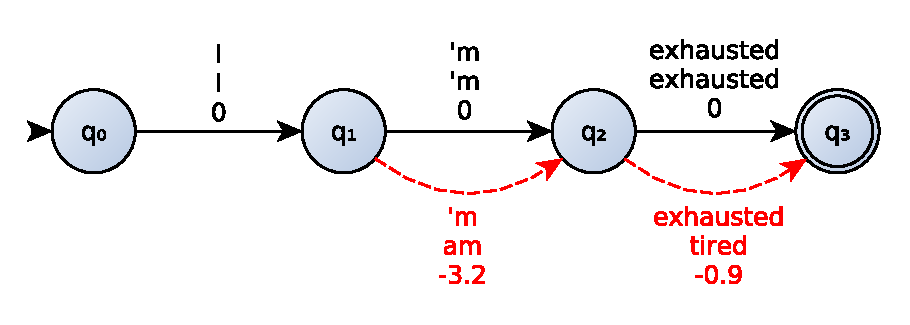
\includegraphics[width=0.7\textwidth]{semirings}
  \caption{An example transducer for the sentence “I'm exhausted”}
  \label{fig:transducer-ex}
\end{figure}

With the monoids defined in \tableref{tab:monoids}, we would obtain
the rewritings shown in \tableref{tab:neglog}. We can clearly observe
the different behaviors of the two monoids in the last row of the
table. While the monoids have similar effects for single
modifications, the desired threshold effect is obtained with Negative
Min and the precise transduction score is retrieved with Negative
Log when considering rewritings with two non-identity transitions.

\begin{table}[H]
  \centering
  \caption{Rewritings of “I'm exhausted”}
  \begin{tabular}[H]{SSl}
    \toprule
    {Negative Log Score} & {Negative Min Score} & {Rewriting} \\
    \midrule
    0 & 0 & I'm exhausted \\
    -0.9 & -0.9 & I'm tired \\
    -3.2 & -3.2 & I am exhausted \\
    -4.1 & -3.2 & I am tired \\
  \end{tabular}
  \label{tab:neglog}
\end{table}

The two monoids are almost usable with the various flavors of score
functions defined in \sectionref{sec:lexical-enhancements}. But since
they are not the log of probabilities, we don't have the guarantee
that $\forall (x, y) \in \mathcal{C}, \mathcal{S}(( x, y)) \in
\mathbb{R}^{-} \cup \{-\infty\}$. To fix this problem and be able to
use the monoids defined above, we normalize the scores by adding
$\argmin_{(x, y) \in \mathcal{C}} \left( \log
  \proba[LM]{x}^{\lambda_2} \right)$ to all the scores computed with
the functions defined in
\sectionref{sec:lexical-enhancements}.

It is now possible to address the two use-cases mentioned in
\figureref{fig:use-cases} by using the Viterbi algorithm
\cite{forney1973viterbi} with Negative Log as monoid for the first
use-case and Negative MaxMin for the second.

The next section details \textsc{Readability Lab}, a framework built
to analyze both the lexical enhancements and the text rewritings
introduced in \sectionref{sec:lexical-enhancements}
and \sectionref{sec:rewriting} in an intuitive and efficient manner.

\section{\textsc{Readability Lab}, a fine-grained readability analysis
  framework}
\label{sec:framework}

To easily assess the quality of the approaches proposed in this work,
a web application has been made available. Creating it was also the
occasion to expose our results to other programs by creating a server
that could easily be used from other tool-chains.

\begin{figure}[h]
  \centering
  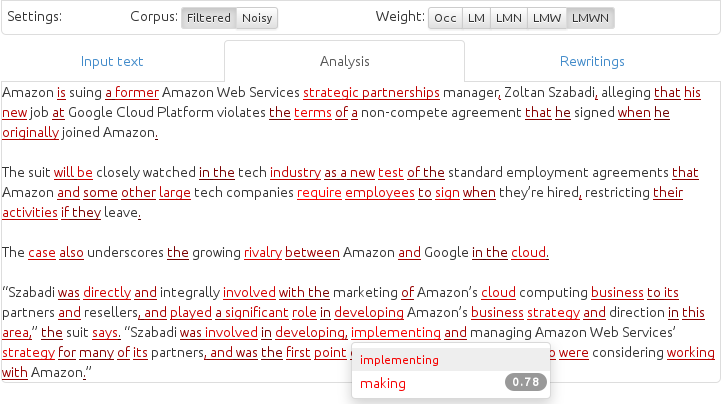
\includegraphics[width=\textwidth]{ui}
  \caption{\textsc{Readability Lab} interface}
  \label{fig:ui}
\end{figure}

\textsc{uimaFIT}, \textsc{Play
  Framework}\footnote{\url{http://www.playframework.com/}},
\textsc{React}\footnote{\url{https://facebook.github.io/react/}} and
\textsc{Heroku}\footnote{\url{https://www.heroku.com/}} were used to
create the application available at
\url{http://readability.crydee.eu/}. \figureref{fig:ui} shows a
screenshot of the interface.

Among the theoretical obstacles faced during the creation of this
demo, the most interesting one is certainly the algorithm used to
detect matches in a text. Indeed, with more than \numprint{30000}
patterns to test, response times easily grow slow. The Aho-Corasick
algorithm was used to address this issue \cite{aho1975efficient}. The
principle of this algorithm is to build an automaton to match a wide
range of patterns that is afterwards usable on any incoming text. The
only unusual aspect in our use of this algorithm is the alphabet we
use: in our case it is the alphabet of pairs of tokens and their part
of speech instead of the classical English alphabet.

This two-step process—slow automaton building and fast searches
afterwards—matches perfectly the structure of a web application where
the starting phase is usually slow, allowing lengthy initialization
processes after which incoming requests have to be handled
promptly. Since no existing implementation that we knew of had
abstracted away the alphabet used, a new implementation has been
proposed that addresses this issue and allows to use arbitrary Java
classes as alphabet (here our pairs of token and their part of
speech). It is freely
available\footnote{\url{https://github.com/m09/aho-corasick}}.

The source of \textsc{Readability Lab} is—yet again—available on
\textsc{Github}\footnote{\url{https://github.com/m09/readability}}.

\chapter{Evaluation \& Discussion}
\label{cha:discussion}

To evaluate and discuss the work proposed in \chapterref{cha:work},
several approaches have been used in the litterature. The main
possibilities are:

\begin{enumerate}
\item the use of machine translation measures, such as BLEU
  \cite{papineni2002bleu}, ROUGE \cite{lin2004rouge} or NIST
  \cite{doddington2002automatic};
\item using readability formulas as scores, including Dale−Chall and
  Flesch Reading Ease;
\item evaluating by comparing agreement among several lexical
  enhancement sources. In their 2010 paper, \cite{yatskar2010sake}
  proposed an evaluation based on a list of interesting rewritings
  built by a \sew{} contributor. However the list does not seem to be
  available anymore;
\item manual evaluation.
\end{enumerate}

Most of these possibilities are flawed in some way: BLEU, ROUGE and
NIST have been built to evaluate a translation from one language to
another. When applied to the same source and target language, their
behavior is sub-optimal at best. To observe this phenomenon, consider
a translation system that does not do anything. In the context of
multilingual translation, it is likely to obtain $0$—the worst
score—with all the metrics mentioned. On the contrary, in the context
of monolingual translation, it might very well obtain very high
scores. Consider the gold translation:

“I went to the park and enjoyed the fantastic weather.” $\rightarrow$
“I went to the park and enjoyed the great weather.”

Compared to it, a NO-OP translation will have a unigram precision of
$\,\sfrac{9}{10}$, a bigram precision of $\,\sfrac{7}{9}$, etc. The
resulting BLEU, ROUGE and NIST scores will be very high. Indeed,
instead of measuring the quality of the translation, they mainly
measure the amount of the sentence that was rewritten.

Readability formulas are also flawed, as detailed
in \chapterref{cha:sota}. A better alternative is to use the most
recent machine learning techniques as baselines, at the price of
implementation troubles.

Finally manual evaluation is flawed in the sense that it either does
not cover a huge amount of data or is not usable in an iterative
testing environment due to the high cost of the process. It also has
the usual problems of annotation—subjectivity and consistency probably
being the main ones.

At the time of this writing, the automatic evaluation is not yet in a
presentable form and we settle for manual evaluation and discussion.

The main point to evaluate in this work is the efficiency of the six
different scoring functions. They are analyzed below. To determine the
problems and advantages of the scoring functions, an empirical study
was led with a range of news articles. This informal insight still has
to be backed up by further experiments at the time of this
writing. All experiments were done with the $\lambda$ parameters fixed
at $1$, which is an obvious problem that will need to be addressed
later on.

\paragraph*{$\mathcal{S}$ \& $\mathcal{S}_c$ functions}
\label{par:occ}

Using a language model to estimate whether or not the word being
rewritten is common already yields interesting results, as shown in
\tableref{tab:tops-socc}. We can note that the $\mathcal{S}_c$
function is subject to a lot of noise. This was to be expected as
there is no measure to ensure that the replacement terms are common in
the English language. More surprising is the score of the “"he
$\rightarrow$ that while giotto” entry given by the $\mathcal{S}$
function. After further investigation, it appears that the term “"he”
has been mistokenized and left as is. Its language model score was
certainly maximal (unknown token) while its length was one, explaining
its very high score.

\begin{table}[H]
  \centering
  \caption{$\mathcal{S}$ \& $\mathcal{S}_c$ top 10 rewritings}
  \noindent\makebox[\textwidth]{%
  \begin{tabularx}{1.1\textwidth}{Sp{1.6cm}p{2.6cm}Sp{2cm}X}
    \toprule
    \multicolumn{3}{c}{{$\mathcal{S}$ function}} & \multicolumn{3}{c}{{$\mathcal{S}_c function$}} \\
    \cmidrule(r{4pt}){1-3} \cmidrule{4-6} \\
    {Score} & Original & Rewriting & {Score} & Original & Rewriting \\
    \midrule
    -9.75  & obtain     & get                &  0.00 & "he           & that while giotto              \\
    -9.79  & discovered & found              & -0.51 & exaggerated   & said that                      \\
    -10.10  & n't        & not               & -0.57 & stray         & wander                         \\
    -10.17  & indicate   & show              & -0.60 & virtuous      & good                           \\
    -10.34  & allow      & let               & -0.64 & discoloration & colour                         \\
    -10.39  & indicate   & show              & -0.66 & :terrorism    & :national liberation movements \\
    -10.43  & fifty-one  & 51                & -0.81 & solely        & only                           \\
    -10.48  & "he        & that while giotto & -0.83 & barrage       & attack                         \\
    -10.53  & resolve    & break             & -0.95 & allow         & make up for                    \\
    -10.54  & entire     & whole             & -0.95 & allow         & let                            \\
  \end{tabularx}}
  \label{tab:tops-socc}
\end{table}

\paragraph*{$\mathcal{S}_d$ \& $\mathcal{S}_{dc}$ functions}
\label{par:sd-sdc}

For those functions, we refer to the appendix \tableref{tab:top-sd}
and \tableref{tab:top-sdc}. Many extremely bad rules reach the top. It
would certainly be interesting—given more time—to adjust the
$\lambda_3$ parameter to reduce the effect of the replacement term
language model score to see if this improves these two functions.

\paragraph*{$\mathcal{S}_{wd}$ \& $\mathcal{S}_{wdc}$ functions}
\label{par:swd}

\tableref{tab:top-swd} \& \tableref{tab:top-swdc} show that allowing
for paraphrases is quite promising: while noisy, these tables have
very interesting rewritings, such as “enact $\rightarrow$ make it into
law” and “unanimously $\rightarrow$ by all of the members”. It would
be extremely hard to come up with one word that has the same meaning
as “enact”, since “enact” is a specialized term. If further study
reveals that it is possible to successfully control the noise with
parameters or extensions to this score function it might become a
worthy candidate for text simplification.

\chapter{Future work}
\label{cha:future-work}

There are many possibilities for future work. Among the most important
ones are:

\begin{enumerate}
\item quantify the impact of the amount of data on the approaches
  proposed. Around \numprint{30000} lexical enhancements, while a good
  start, is certainly a number that could grow with great effects for
  our statistical approaches;
\item better handle grammaticality in the lexical rewriting context by
  using syntactic parsing information to constrain rewritings is a
  promising possibility;
\item investigate syntactic readability issues in the fine-grained
  analysis context, in particular by going from a string to string
  transduction process to a tree to tree transduction process,
  following related work in text rewriting;
\item integrate gaze information in the process of estimating the
  readability of an area of a text. It should combine especially well
  with lexical estimations, because both can be anchored precisely in
  a text. Conversely, it might be more challenging to improve a
  syntactic approach with gaze information.
\item conduct a thorough evaluation, including automatic evaluation
  with readability measures, lexical improvement lists comparison and
  manual evaluation. An idea to evaluate manually the quality of the
  rewritings proposed is to submit two rewritings, one of our own and
  one of a similar approach to a human judge together with the
  original text being rewritten and ask the judge to compare the two
  rewritings.
\end{enumerate}

During the month left of this internship, we plan on focusing on tree
transducing (3.) and a better evaluation (5.).

\chapter{Conclusion}

In this work we studied how to extend classical machine translation
and readability techniques to obtain fine-grained measurements of the
readability of a text. We also explored the related tasks of text
rewriting.

Despite the lack of a proper evaluation, the tool created to estimate
the interest of our approaches—\textsc{Readability Lab}—already allows
users to get feedback on any written text using our methods.

On a personal level, I learned a lot during this internship. It
allowed me to explore many aspects of gaze processing, readability,
machine translation and the theories those domains are based on, such
as string and tree transducing. By implementing a fairly large
software solution around these problems I also gained more knowledge
of the NLP software eco-system, which is always very interesting for a
NLP student. I would like to mention that topics such as math
information retrieval and scientific paper analysis during the weekly
meetings of \textsc{Aizawa Laboratory} was very interesting as well.

This internship was also my first contact with a long-term research
activity. It was very challenging to correctly balance theoretical
work and implementation and I am happy to have been able to experience
that as it will help me for my future activities.

I also noticed that it is hard to properly conceptualize “all day
every day” during a research activity. Writing this report has brought
many concepts and improvements that I had not thought of before trying
to get the whole system on paper. It also appeared to me that I had
reinvented the wheel many times over the course of this internship and
it is a good experience to have, so that it can be avoided in the
future and replaced by adequate search of existing literature.

As a final note to this internship report, I would like to thank
\textsc{Aizawa-sensei} again for her support during this internship,
it was great to be a part of \textsc{Aizawa Laboratory} during those
five months.

\bibliographystyle{apalike2}
\bibliography{report.bib}

\appendix

\chapter{Open source contributions}
\label{cha:oss-contribs}

During this internship I had the opportunity to contribute to the open
source natural language processing community. What follows is a list
of those contributions. When no link is provided, the software is part
of the \textsc{Readability Lab} repository already linked several
times in this report.

\section{Enhancements of existing software}
\label{sec:enhancements}

\begin{itemize}
\item
  \href{https://bugs.eclipse.org/bugs/show_bug.cgi?id=433163}{Wikitext
    parser bug filing}
\item \href{https://issues.apache.org/jira/browse/OPENNLP-676}{OpenNLP
    POSTagger bug filing with patch}
\item \href{https://issues.apache.org/jira/browse/UIMA-3913}{uimaFIT
    enhancement proposal}
\end{itemize}

\section{\textsc{uimaFIT} components}
\label{sec:uimafit-components}

\begin{itemize}
\item sentence alignment analysis engine, using Myers' algorithm
\item word alignment analysis engine, using yet again Myers' algorithm
\item \href{https://berkeleylm.googlecode.com/}{BerkeleyLM} uimaFIT
  wrapper
\item readability formulas uimaFIT calculator
\end{itemize}

\section{Miscellaneous}
\label{sec:misc-software}
\begin{itemize}
\item Wikimedia PostgreSQL importer
\item Generic implementation of Aho-Corasick
\end{itemize}

\chapter{Top rewritings}

\section{Top 30 for the score function $\mathcal{S}$}
\begin{table}[H]
  \centering
  \caption{$\mathcal{S}$ top 30 rewritings}
  \begin{tabularx}{\textwidth}{SXX}
    \toprule
    {Score} & Original & Revised \\
    \midrule
    -9.75 & obtain & get \\
    -9.79 & discovered & found \\
    -10.10 & n't & not \\
    -10.17 & indicate & show \\
    -10.34 & allow & let \\
    -10.39 & indicate & show \\
    -10.43 & fifty-one & 51 \\
    -10.48 & "he & that while giotto \\
    -10.53 & resolve & break \\
    -10.54 & entire & whole \\
    -10.62 & incredibly & very \\
    -10.68 & invitees & players they invited \\
    -10.68 & commenced & started \\
    -10.71 & created & made \\
    -10.78 & digit & number \\
    -10.83 & preserve & keep \\
    -10.93 & inducted & added \\
    -10.95 & assumed & thought \\
    -10.97 & relocated & moved \\
    -10.97 & castaway & player \\
    -11.00 & exaggerated & said that \\
    -11.01 & prevent & stop \\
    -11.06 & stray & wander \\
    -11.09 & virtuous & good \\
    -11.13 & discoloration & colour \\
    -11.14 & amended & changed \\
    -11.15 & :terrorism & :national liberation movements \\
    -11.21 & remain & stay \\
    -11.22 & entente & allies \\
    -11.24 & suitable & good \\

  \end{tabularx}
\end{table}

\section{Top 30 for the score function $\mathcal{S}_c$}
\begin{table}[H]
  \centering
  \caption{$\mathcal{S}_c$ top 30 rewritings}
  \begin{tabularx}{\textwidth}{SXX}
    \toprule
    {Score} & Original & Revised \\
    \midrule
     0.00 & "he & that while giotto \\
    -0.51 & exaggerated & said that \\
    -0.57 & stray & wander \\
    -0.60 & virtuous & good \\
    -0.64 & discoloration & colour \\
    -0.66 & :terrorism & :national liberation movements \\
    -0.81 & solely & only \\
    -0.83 & barrage & attack \\
    -0.95 & allow & make up for \\
    -0.95 & allow & let \\
    -0.98 & marketed & sold \\
    -1.02 & notebook & laptop \\
    -1.02 & cooperate & work well \\
    -1.04 & boasts & has \\
    -1.05 & obtain & get \\
    -1.06 & reflected & shown \\
    -1.06 & reflected & showed \\
    -1.09 & township & town \\
    -1.16 & assumed & thought \\
    -1.18 & inh & in \\
    -1.18 & authoritative & sacred \\
    -1.20 & sub-discipline & kind \\
    -1.21 & recedes & drains \\
    -1.26 & lowered & became cheaper \\
    -1.29 & cups & being prepared \\
    -1.29 & sterilise & sterilize \\
    -1.29 & indicate & show \\
    -1.29 & indicate & show \\
    -1.29 & commissions & pays for \\
    -1.29 & combatants & fighters \\
  \end{tabularx}
\end{table}

\section{Top 30 for the score function $\mathcal{S}_d$}
\begin{table}[H]
  \centering
  \caption{$\mathcal{S}_d$ top 30 rewritings}
  \begin{tabularx}{\textwidth}{SXX}
    \toprule
    {Score} & Original & Revised \\
    \midrule
    -15.27 & ; & . \\
    -15.41 & , & . \\
    -15.57 & and & . \\
    -16.06 & ,but & . \\
    -16.98 & ,and & . \\
    -17.29 & : & . \\
    -17.35 & inh & in \\
    -17.51 & where & . \\
    -17.52 & n't & not \\
    -17.71 & ''the & the \\
    -17.77 & speedminton & it \\
    -17.78 & so-called & . \\
    -17.80 & with & . \\
    -17.81 & incredibly & very \\
    -17.95 & involved & . \\
    -18.02 & satisfy & the \\
    -18.02 & obtain & get \\
    -18.03 & , and & . \\
    -18.07 & gws & it \\
    -18.18 & solely & only \\
    -18.28 & which & . \\
    -18.28 & allow & let \\
    -18.29 & ,<ref & .<ref \\
    -18.29 & while & . \\
    -18.30 & - & . \\
    -18.36 & incident & , \\
    -18.38 & included & . \\
    -18.43 & "at & in \\
    -18.44 & ,<ref & .<ref \\
    -18.48 & redone & new \\
  \end{tabularx}
  \label{tab:top-sd}
\end{table}

\section{Top 30 for the score function $\mathcal{S}_{dc}$}
\begin{table}[H]
  \centering
  \caption{$\mathcal{S}_{dc}$ top 30 rewritings}
  \begin{tabularx}{\textwidth}{SXX}
    \toprule
    {Score} & Original & Revised \\
    \midrule
    -5.57 & ,but & . \\
    -6.86 & inh & in \\
    -7.19 & ,and & . \\
    -7.22 & ''the & the \\
    -7.28 & speedminton & it \\
    -7.53 & satisfy & the \\
    -7.69 & solely & only \\
    -7.94 & "at & in \\
    -8.02 & ...the & the \\
    -8.09 & tribe & " \\
    -8.09 & m13 & it \\
    -8.10 & virtuous & good \\
    -8.12 & greengard & he \\
    -8.12 & waned with & . \\
    -8.14 & outlive & after \\
    -8.14 & enterprising & some \\
    -8.15 & involved & . \\
    -8.20 & mcewen & it \\
    -8.25 & townsfolk & people \\
    -8.25 & orators & people \\
    -8.31 & wary & because \\
    -8.39 & rations & they \\
    -8.39 & tinsulanonda & he \\
    -8.47 & naiad & it \\
    -8.47 & itis & it is \\
    -8.47 & motions & even \\
    -8.48 & foregoing & at \\
    -8.54 & referenes & references \\
    -8.55 & democide & people \\
    -8.56 & incident & , \\
  \end{tabularx}
  \label{tab:top-sdc}
\end{table}

\section{Top 30 for the score function $\mathcal{S}_{wd}$}
\begin{table}[H]
  \centering
  \caption{$\mathcal{S}_{wd}$ top 30 rewritings}
  \begin{tabularx}{\textwidth}{SXX}
    \toprule
    {Score} & Original & Revised \\
    \midrule
    -14.20 & investigate & see if it was true \\
    -15.07 & "he & that while giotto \\
    -15.08 & enact & make it into law. \\
    -15.21 & :terrorism & :national liberation movements \\
    -15.26 & a/k/a & , also known as \\
    -15.27 & invitees & players they invited \\
    -15.27 & ; & . \\
    -15.33 & allow & make up for \\
    -15.34 & indulgence & doing what you want, \\
    -15.34 & unanimously & by all of the members \\
    -15.41 & , & . \\
    -15.45 & exaggerated & said that \\
    -15.45 & cosmography & the world and the universe \\
    -15.50 & straddles & built on the banks of \\
    -15.55 & favorably & in a good way \\
    -15.57 & consisted & was made up \\
    -15.57 & and & . \\
    -15.60 & society- & society, such as \\
    -15.61 & centralised & put into one place, \\
    -15.61 & potable & the country's \\
    -15.64 & oxygen-carrying & proteins in the baby's \\
    -15.68 & nationalteams & national team in norway \\
    -15.69 & spans & 's a bit longer than \\
    -15.70 & phenotype & strength of natural selection \\
    -15.79 & hfcs & high fructose corn syrup \\
    -15.79 & hfcs & high fructose corn syrup \\
    -15.80 & exclusively & all the time \\
    -15.81 & negligible & "not needed" \\
    -15.81 & befriended & became friends with \\
    -15.83 & vice-versa & the other way round \\
  \end{tabularx}
  \label{tab:top-swd}
\end{table}

\section{Top 30 for the score function $\mathcal{S}_{wdc}$}
\begin{table}[H]
  \centering
  \caption{$\mathcal{S}_{wdc}$ top 30 rewritings}
  \begin{tabularx}{\textwidth}{SXX}
    \toprule
    {Score} & Original & Revised \\
    \midrule
    -4.58 & "he & that while giotto \\
    -4.59 & enact & make it into law. \\
    -4.72 & :terrorism & :national liberation movements \\
    -4.77 & a/k/a & , also known as \\
    -4.84 & allow & make up for \\
    -4.85 & indulgence & doing what you want, \\
    -4.85 & unanimously & by all of the members \\
    -4.96 & exaggerated & said that \\
    -4.96 & cosmography & the world and the universe \\
    -5.01 & straddles & built on the banks of \\ 
    -5.06 & favorably & in a good way \\
    -5.10 & investigate & see if it was true \\
    -5.11 & society- & society, such as \\
    -5.12 & centralised & put into one place, \\
    -5.16 & oxygen-carrying & proteins in the baby's \\
    -5.19 & nationalteams & national team in norway \\
    -5.21 & phenotype & strength of natural selection \\
    -5.30 & hfcs & high fructose corn syrup \\
    -5.30 & hfcs & high fructose corn syrup \\
    -5.32 & negligible & "not needed" \\
    -5.32 & befriended & became friends with \\
    -5.34 & vice-versa & the other way round \\
    -5.34 & eschewed & did not focus on \\
    -5.37 & purportedly & said to have been \\
    -5.39 & exemplified & was part of \\
    -5.39 & itis & it is \\
    -5.41 & cohuna & pleistocene burials have been found \\
    -5.43 & resented & did not like \\
    -5.44 & remediation & damage that should be fixed \\
    -5.44 & precedes & in front of \\
  \end{tabularx}
  \label{tab:top-swdc}
\end{table}

\end{document}
%%% Local Variables: 
%%% coding: utf-8
%%% mode: latex
%%% TeX-engine: xetex
%%% End: 
